\documentclass[preview,border=7pt]{standalone}
\usepackage{amsmath,amssymb,xcolor}
\usepackage{tikz}
\usetikzlibrary{arrows.meta}
\definecolor{acc}{RGB}{47,143,132}
\definecolor{cyn}{RGB}{6,182,212}
\definecolor{amb}{RGB}{245,158,11}
\begin{document}
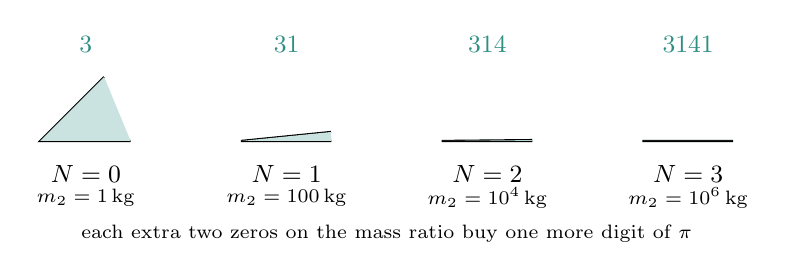
\begin{tikzpicture}
\definecolor{blu}{RGB}{96,165,250}
%% N=0, θ=π/4
\begin{scope}[shift={(0,0)}]
\draw[line width=.8pt] (1.15,0) -- (0,0) -- ({1.15*cos(45)},{1.15*sin(45)});
\fill[acc!25] (0,0) -- (1.15,0) -- ({1.15*cos(45)},{1.15*sin(45)}) -- cycle;
\node at (0.58,-0.42) {\small $N=0$};
\node at (0.58,-0.72) {\scriptsize $m_2=1\,\mathrm{kg}$};
\node[acc] at (0.58,1.22) {\small $3$};
\end{scope}
%% N=1, θ=arctan(0.1) ≈ 5.71°
\begin{scope}[shift={(2.55,0)}]
\draw[line width=.8pt] (1.15,0) -- (0,0) -- ({1.15*cos(5.711)},{1.15*sin(5.711)});
\fill[acc!25] (0,0) -- (1.15,0) -- ({1.15*cos(5.711)},{1.15*sin(5.711)}) -- cycle;
\node at (0.58,-0.42) {\small $N=1$};
\node at (0.58,-0.72) {\scriptsize $m_2=100\,\mathrm{kg}$};
\node[acc] at (0.58,1.22) {\small $31$};
\end{scope}
%% N=2, θ=arctan(0.01) ≈ 0.573°
\begin{scope}[shift={(5.10,0)}]
\draw[line width=.8pt] (1.15,0) -- (0,0) -- ({1.15*cos(0.573)},{1.15*sin(0.573)});
\fill[acc!35] (0,0) -- (1.15,0) -- ({1.15*cos(0.573)},{1.15*sin(0.573)}) -- cycle;
\node at (0.58,-0.42) {\small $N=2$};
\node at (0.58,-0.72) {\scriptsize $m_2=10^{4}\,\mathrm{kg}$};
\node[acc] at (0.58,1.22) {\small $314$};
\end{scope}
%% N=3, θ=arctan(0.001) ≈ 0.0573°
\begin{scope}[shift={(7.65,0)}]
\draw[line width=.8pt] (1.15,0) -- (0,0) -- ({1.15*cos(0.0573)},{1.15*sin(0.0573)});
\fill[acc!45] (0,0) -- (1.15,0) -- ({1.15*cos(0.0573)},{1.15*sin(0.0573)}) -- cycle;
\node at (0.58,-0.42) {\small $N=3$};
\node at (0.58,-0.72) {\scriptsize $m_2=10^{6}\,\mathrm{kg}$};
\node[acc] at (0.58,1.22) {\small $3141$};
\end{scope}
\node at (4.40,-1.18) {\scriptsize each extra two zeros on the mass ratio buy one more digit of $\pi$};
\end{tikzpicture}
\end{document}
